%%%%%%%%%%%%%%%%%%%%%%%%%%%%%%%%%%%%%%%%%
% Beamer Presentation
% LaTeX Template
% Version 2.0 (March 8, 2022)
%
% This template originates from:
% https://www.LaTeXTemplates.com
%
% Author:
% Vel (vel@latextemplates.com)
%
% License:
% CC BY-NC-SA 4.0 (https://creativecommons.org/licenses/by-nc-sa/4.0/)
%
%%%%%%%%%%%%%%%%%%%%%%%%%%%%%%%%%%%%%%%%%

%----------------------------------------------------------------------------------------
%	PACKAGES AND OTHER DOCUMENT CONFIGURATIONS
%----------------------------------------------------------------------------------------

\documentclass[
	11pt, % Set the default font size, options include: 8pt, 9pt, 10pt, 11pt, 12pt, 14pt, 17pt, 20pt
	%t, % Uncomment to vertically align all slide content to the top of the slide, rather than the default centered
	%aspectratio=169, % Uncomment to set the aspect ratio to a 16:9 ratio which matches the aspect ratio of 1080p and 4K screens and projectors
]{beamer}

\graphicspath{../Figures/} % Specifies where to look for included images (trailing slash required)

\usepackage{booktabs} % Allows the use of \toprule, \midrule and \bottomrule for better rules in tables

%----------------------------------------------------------------------------------------
%	SELECT LAYOUT THEME
%----------------------------------------------------------------------------------------

% Beamer comes with a number of default layout themes which change the colors and layouts of slides. Below is a list of all themes available, uncomment each in turn to see what they look like.

%\usetheme{default}
%\usetheme{AnnArbor}
%\usetheme{Antibes}
%\usetheme{Bergen}
%\usetheme{Berkeley}
%\usetheme{Berlin}
%\usetheme{Boadilla}
%\usetheme{CambridgeUS}
%\usetheme{Copenhagen}
%\usetheme{Darmstadt}
%\usetheme{Dresden}
%\usetheme{Frankfurt}
%\usetheme{Goettingen}
\usetheme{Hannover}%ok
%\usetheme{Ilmenau}
%\usetheme{JuanLesPins}
%\usetheme{Luebeck}
%\usetheme{Madrid}
%\usetheme{Malmoe}
%\usetheme{Marburg}
%\usetheme{Montpellier}
%\usetheme{PaloAlto}
%\usetheme{Pittsburgh}
%\usetheme{Rochester}
%\usetheme{Singapore}
%\usetheme{Szeged}
%\usetheme{Warsaw}


%----------------------------------------------------------------------------------------
%	SELECT COLOR THEME
%----------------------------------------------------------------------------------------

% Beamer comes with a number of color themes that can be applied to any layout theme to change its colors. Uncomment each of these in turn to see how they change the colors of your selected layout theme.

%\usecolortheme{albatross}
%\usecolortheme{beaver}
%\usecolortheme{beetle}
%\usecolortheme{crane}
%\usecolortheme{dolphin}
%\usecolortheme{dove}
%\usecolortheme{fly}
%\usecolortheme{lily}
%\usecolortheme{monarca}
%\usecolortheme{seagull}
%\usecolortheme{seahorse}
%\usecolortheme{spruce}
%\usecolortheme{whale}
%\usecolortheme{wolverine}

%----------------------------------------------------------------------------------------
%	SELECT FONT THEME & FONTS
%----------------------------------------------------------------------------------------

% Beamer comes with several font themes to easily change the fonts used in various parts of the presentation. Review the comments beside each one to decide if you would like to use it. Note that additional options can be specified for several of these font themes, consult the beamer documentation for more information.

\usefonttheme{default} % Typeset using the default sans serif font
%\usefonttheme{serif} % Typeset using the default serif font (make sure a sans font isn't being set as the default font if you use this option!)
%\usefonttheme{structurebold} % Typeset important structure text (titles, headlines, footlines, sidebar, etc) in bold
%\usefonttheme{structureitalicserif} % Typeset important structure text (titles, headlines, footlines, sidebar, etc) in italic serif
%\usefonttheme{structuresmallcapsserif} % Typeset important structure text (titles, headlines, footlines, sidebar, etc) in small caps serif

%------------------------------------------------

%\usepackage{mathptmx} % Use the Times font for serif text
\usepackage{palatino} % Use the Palatino font for serif text
\usepackage{listings}
%\usepackage{helvet} % Use the Helvetica font for sans serif text
\usepackage[default]{opensans} % Use the Open Sans font for sans serif text
%\usepackage[default]{FiraSans} % Use the Fira Sans font for sans serif text
%\usepackage[default]{lato} % Use the Lato font for sans serif text
\usepackage{xcolor}
\usepackage{graphicx}
\usepackage[T1]{fontenc}
   \logo{
\includegraphics[height=1.5cm]{../Figures/redif_logo.jpeg}}
\definecolor{codegreen}{rgb}{0,0.6,0}
\definecolor{codegray}{rgb}{0.5,0.5,0.5}
\definecolor{codepurple}{rgb}{0.58,0,0.82}
\definecolor{backcolour}{rgb}{0.95,0.95,0.92}

\lstdefinestyle{mystyle}{
    backgroundcolor=\color{backcolour},    
    commentstyle=\color{codegreen},
    keywordstyle=\color{magenta},
    numberstyle=\tiny\color{codegray},
    stringstyle=\color{codepurple},
    basicstyle=\ttfamily\footnotesize,
    breakatwhitespace=false,         
    breaklines=true,                 
    captionpos=b,                    
    keepspaces=true,                 
    numbers=left,                    
    numbersep=5pt,                  
    showspaces=false,                
    showstringspaces=false,
    showtabs=false,                  
    tabsize=2
}

\lstset{style=mystyle}

\setbeamertemplate{navigation symbols}{\insertlogo}


%----------------------------------------------------------------------------------------
%	SELECT INNER THEME
%----------------------------------------------------------------------------------------

% Inner themes change the styling of internal slide elements, for example: bullet points, blocks, bibliography entries, title pages, theorems, etc. Uncomment each theme in turn to see what changes it makes to your presentation.

%\useinnertheme{default}
\useinnertheme{circles}
%\useinnertheme{rectangles}
%\useinnertheme{rounded}
%\useinnertheme{inmargin}

%----------------------------------------------------------------------------------------
%	SELECT OUTER THEME
%----------------------------------------------------------------------------------------

% Outer themes change the overall layout of slides, such as: header and footer lines, sidebars and slide titles. Uncomment each theme in turn to see what changes it makes to your presentation.

%\useoutertheme{default}
%\useoutertheme{infolines}
%\useoutertheme{miniframes}
%\useoutertheme{smoothbars}
%\useoutertheme{sidebar}
%\useoutertheme{split}
%\useoutertheme{shadow}
%\useoutertheme{tree}
%\useoutertheme{smoothtree}

%\setbeamertemplate{footline} % Uncomment this line to remove the footer line in all slides
%\setbeamertemplate{footline}[page number] % Uncomment this line to replace the footer line in all slides with a simple slide count

%\setbeamertemplate{navigation symbols}{} % Uncomment this line to remove the navigation symbols from the bottom of all slides

%----------------------------------------------------------------------------------------
%	PRESENTATION INFORMATION
%----------------------------------------------------------------------------------------

\title[RedIF 2022]{Introduction to mrgsolve :  \\Hands on tutorial} % The short title in the optional parameter appears at the bottom of every slide, the full title in the main parameter is only on the title page

%\subtitle{Optional Subtitle} % Presentation subtitle, remove this command if a subtitle isn't required

\author[Kyle Baron \and Ana Ruiz]{Kyle Baron and Ana Ruiz} % Presenter name(s), the optional parameter can contain a shortened version to appear on the bottom of every slide, while the main parameter will appear on the title slide

\institute{Metrum Research Group and Gilead Sciences} % Your institution, the optional parameter can be used for the institution shorthand and will appear on the bottom of every slide after author names, while the required parameter is used on the title slide and can include your email address or additional information on separate lines


\date[\today]{Red Iberoamericana de Farmacometria 2022 \\ \today} % Presentation date or conference/meeting name, the optional parameter can contain a shortened version to appear on the bottom of every slide, while the required parameter value is output to the title slide

%----------------------------------------------------------------------------------------

\begin{document}

%----------------------------------------------------------------------------------------
%	TITLE SLIDE
%----------------------------------------------------------------------------------------

\begin{frame}
	\titlepage % Output the title slide, automatically created using the text entered in the PRESENTATION INFORMATION block above



\end{frame}




%----------------------------------------------------------------------------------------
%	TABLE OF CONTENTS SLIDE
%----------------------------------------------------------------------------------------

% The table of contents outputs the sections and subsections that appear in your presentation, specified with the standard \section and \subsection commands. You may either display all sections and subsections on one slide with \tableofcontents, or display each section at a time on subsequent slides with \tableofcontents[pausesections]. The latter is useful if you want to step through each section and mention what you will discuss.

\begin{frame}
	\frametitle{Presentation Overview} % Slide title, remove this command for no title
	
	\tableofcontents % Output the table of contents (all sections on one slide)
	%\tableofcontents[pausesections] % Output the table of contents (break sections up across separate slides)
\end{frame}

%----------------------------------------------------------------------------------------
%	PRESENTATION BODY SLIDES
%----------------------------------------------------------------------------------------
\begin{frame}
\frametitle{The Brain}
	\framesubtitle{Kyle Baron, Science Advisor, Principal Scientist II at Metrum Research Group}
\begin{figure}
   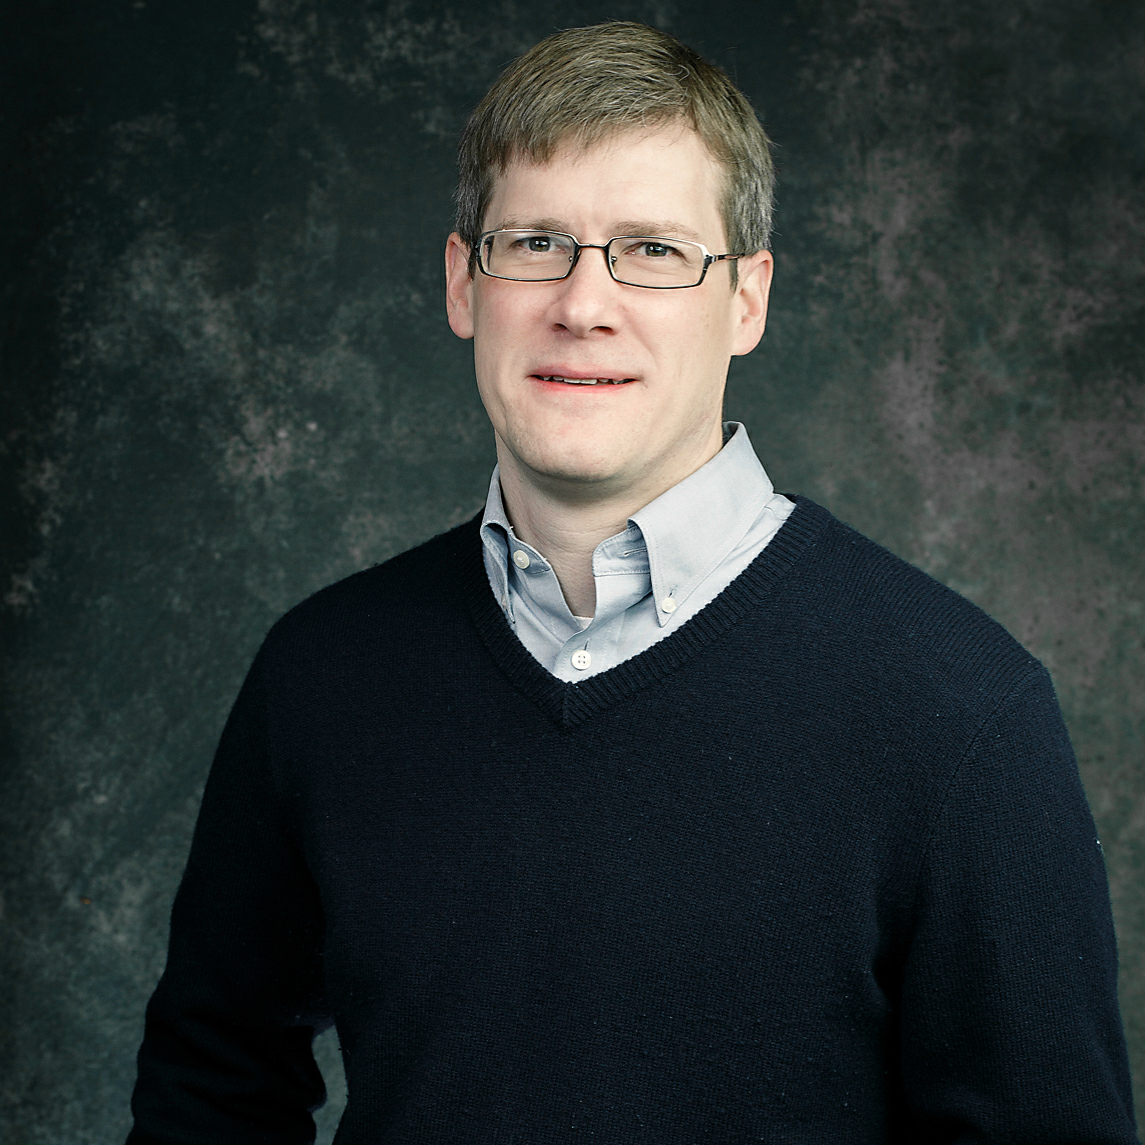
\includegraphics[width= 0.55\linewidth]{../Figures/kyle.jpg}
\end{figure}


\end{frame}





%--------------------------------------------------------------------------

\section{R Basics} % Sections are added in order to organize your presentation into discrete blocks, all sections and subsections are automatically output to the table of contents as an overview of the talk but NOT output in the presentation as separate slides

% %------------------------------------------------


\subsection{What is R?}
\begin{frame}[fragile]{What is R?}
	\frametitle{What is R?}
	\framesubtitle{Introduction} % Optional subtitle
    \begin{block}{}
	\begin{itemize}
\small
\item R is a language and environment for statistical computing and graphics. 

\item R provides a wide variety of statistical and graphical techniques, and is highly extensible. R provides an Open Source route to participation in that activity.

\item Well-designed publication-quality plots can be produced while user retains full control.

\item R is available as Free Software under the terms of the Free Software Foundation’s GNU General Public License in source code form. It compiles and runs on a wide variety of UNIX platforms, Windows and MacOS.

\item More information can be found at:\href{hhtp://r-project.org/}{\beamergotobutton{hhtp://r-project.org/}}



\end{itemize}

	\end{block}
	
	\end{frame}
	
%--------------------------------------------------------	
\subsection{RStudio}
\begin{frame}[fragile]{RStudio}
	\frametitle{RStudio}
	\framesubtitle{To posit means to put forth an idea for discussion} % Optional subtitle
    \begin{block}{}
	\begin{itemize}
\small
\item \textbf{RStudio Workbench} is an integrated development environment for R and Python, with a console, syntax-highlighting editor that supports direct code execution, history, debugging and workspace management. 

\item \textbf{RStudio Cloud} is a lightweight, cloud-based solution that allows anyone to do, share, teach and learn data science online.

\item \textbf{RStudio Connect} allows you to share data products across your organization (Shiny applications, R Markdown reports, Jupyter Notebooks, and more).

\item \textbf{RStudio Package Manager} will allow you to control, organize, and govern your use of R packages.



\end{itemize}

	\end{block}
	
	\end{frame}
	


%------------------------------------------------

\subsection{Command Line}
\begin{frame}[fragile]{Command Line}
	\frametitle{Command Line}
	\framesubtitle{R packages and more} % Optional subtitle

	\begin{block}{Installing packages}
\begin{lstlisting}[language=R]
install.packages("tidyverse")
library(tidyverse)
update.packages("tidyverse")
\end{lstlisting}
     \vskip0pt 
	\end{block}
		\begin{block}{Getting help}
\begin{lstlisting}[language=R]
help("mutate")
?mutate
example(mutate)
\end{lstlisting}
     \vskip0pt 
	\end{block}

\end{frame}

%------------------------------------------------
%------------------------------------------------


\begin{frame}[fragile]{Command Line}
	\frametitle{Command Line}
	\framesubtitle{Paths} % Optional subtitle

\begin{block}{Paths}
\begin{lstlisting}[language=R]
.GlobalEnv or globalenv()
sessionInfo()
.libPaths()
setwd("/cloud/project/script")
getwd()
\end{lstlisting}
     \vskip0pt 
	\end{block}

\end{frame}

%---------------------------------------
% 

\begin{frame}[fragile]{Command Line}
	\frametitle{Command Line}
	\framesubtitle{Open/Save objects} % Optional subtitle

\begin{block}{Open/Save objects}
\begin{lstlisting}[language=R]
read.csv(file="example.csv",na=".")
read.table("test.csv", sep=",", header=TRUE, skip=1,as.is=TRUE)
write.csv(d,"test.csv",quote=F,na=".",row.names = F)
\end{lstlisting}
     \vskip0pt 
	\end{block}

\end{frame}

%------------------------------------------------
\subsection{Tidyverse}
\begin{frame}[fragile]{Tydiverse}
	\frametitle{Tidyverse}
	\framesubtitle{Learning Tidy} % Optional subtitle

	\begin{columns}[c] % The "c" option specifies centered vertical alignment while the "t" option is used for top vertical alignment
		\begin{column}{0.65\textwidth} % Left column width
			\textbf{Learning Tidy}
			\begin{itemize}
        \item The tidyverse is an opinionated collection of R packages designed for data science. All packages share       an underlying design philosophy, grammar, and data structures.
        \item Following three rules makes a dataset tidy: variables are in columns, observations are in rows, and values are in cells.

           \item “R for Data Science”. Read it online at \href{https://r4ds.had.co.nz/}{\beamergotobutton{R for Data Science}}
			\end{itemize}
		\end{column}
		\begin{column}{0.35\textwidth} % Right column width
\begin{figure}
   
\includegraphics[width= 0.6\linewidth]{../Figures/tidyverse.png}
\end{figure}
		\end{column}
	\end{columns}
	
	\end{frame}
	
%------------------------------------------------
\subsection{Data}
\begin{frame}[fragile]{Data}
	\frametitle{Data}
	\framesubtitle{Basic Types} % Optional subtitle
 \begin{block}{Basic Types}
	 R has six basic (‘atomic’) data types: logical, numeric, integer, complex, string (or character) and raw. The modes and storage modes for the different vector types are listed in the following table.
			\begin{itemize}
			\small
        \item \textbf{logical}: logical data (TRUE or FALSE). Also known as boolean data type, it can only take 2 values
        \item \textbf{numeric}: all real numbers with or without decimal values
        \item \textbf{integer}: real values without decimal points
        \item \textbf{complex}: purely imaginary values (3+2i)
        \item \textbf{character}: character strings values
        \item \textbf{raw}: (unususal) specifies values as raw bytes
			\end{itemize}
	\end{block}
			\end{frame}


%------------------------------------------------

 \begin{frame}
	\frametitle{Data}
	\framesubtitle{Data Objects} % Optional subtitle
 \begin{block}{Data Objects}
		Vectors and factors are built using atomic data types.	Vectors can be thought of as contiguous cells containing data. Cells are accessed through indexing operations such as x[5].
			\begin{itemize}
			\small
        \item \textbf{vector}: a list of atomic values
        \item \textbf{factor}: variables that can take on a limited number of different values. This relates to the concept of levels, where the level of a factor is basically the number of distinct elements
			\end{itemize}
	\end{block}
			\end{frame}
%------------------------------------------------
\subsection{Piping}
\begin{frame}[fragile]{Piping}
	\frametitle{Piping}
	\framesubtitle{magrittr} % Optional subtitle

	\begin{columns}[c] % The "c" option specifies centered vertical alignment while the "t" option is used for top vertical alignment
		\begin{column}{0.75\textwidth} % Left column width
			\textbf{magrittr}
			\begin{itemize}
        \item Pipes are an extremely useful tool from the magrittr package 1 that allow you to express a sequence of multiple operations. They can greatly simplify your code and make your operations more intuitive. However they are not the only way to write your code and combine multiple operations.
        \item \textbf{open R file datamanipulation}
			\end{itemize}
		  
		\end{column}
		\begin{column}{0.25\textwidth} % Right column width
\begin{figure}
   
\includegraphics[width= 0.9\linewidth]{../Figures/pipe.jpg}
\end{figure}
		\end{column}
	\end{columns}
	\end{frame}
%------------------------------------------------
\subsection{ggplot2}
\begin{frame}[fragile]{ggplot2}
	\frametitle{ggplot2}
	\framesubtitle{Data visualization} % Optional subtitle

	\begin{columns}[c] % The "c" option specifies centered vertical alignment while the "t" option is used for top vertical alignment
		\begin{column}{0.75\textwidth} % Left column width
			\textbf{Data visualization}
			\begin{itemize}
			\small
        \item ggplot2 is a system for declaratively creating graphics, based on The Grammar of Graphics. You provide the data, tell ggplot2 how to map variables to aesthetics, what graphical primitives to use, and it takes care of the details.
        \item The \textcolor{codegreen}{Data Visualisation} and \textcolor{codegreen}{Graphics for communication} chapters in R for Data Science will get you up to speed with the essentials of ggplot2 as quickly as possible.
        \item cheat sheet included under Documents (data-visualization-2.1.pdf)
        \item \textbf{open R file ggplot2}
			\end{itemize}
		\end{column}
		\begin{column}{0.25\textwidth} % Right column width
\begin{figure}
   
\includegraphics[width= 0.7\linewidth]{../Figures/ggplot2.png}
\end{figure}
		\end{column}
	\end{columns}
	
	\end{frame}
%------------------------------------------------

\section{Starting with mrgsolve}


\subsection{Introduction}
\begin{frame}[fragile]{Introduction}
	\frametitle{Introduction}
	\framesubtitle{} % Optional subtitle
	\begin{columns}[c] 
		\begin{column}{0.75\textwidth}
	\begin{block}{mrgsolve}
	\small
	\begin{itemize}
		\item mrgsolve is an R package for simulation from hierarchical, ordinary differential equation (ODE) based models typically employed in drug development. mrgsolve has been used for a wide variety of model applications, including pharamacokinetics (PK), pharmacokinetics/pharmacodynamics (PK/PD), physiologically-based pharmacokinetic (PBPK) modeling, and quantitative systems pharmacology. 
		\item mrgsolve is is free, open-source software.
		\end{itemize}
	\end{block}
	\end{column}
		\begin{column}{0.25\textwidth} % Right column width
\begin{figure}
   
\includegraphics[width= 0.7\linewidth]{../Figures/MRG-Solve-Hex.png}
\end{figure}
		\end{column}
	\end{columns}
	\end{frame}
	
%-----------------------------------




\subsection{Online Resources}
\begin{frame}[fragile]{Online Resources}
  \frametitle{Online Resources}
    \begin{block}{Online Resources}
      \begin{itemize}
         \item \href{https://mrgsolve.org/}{\beamergotobutton{mrgsolve}}, this website includes:
           \begin{itemize}
           \item User Guide
           \item Package documentation
           \item R documentation
           \item Doxygen documentation
           \item Vignettes
           \item Demos
           \end{itemize}
        \item \href{https://github.com/metrumresearchgroup/mrgsolve}{\beamergotobutton{mrgsolve github}}A github repository of short, focused, how-to vignettes
      \end{itemize}
    \end{block}

\end{frame}
%------------------------------------------------------
\subsection{Model Specification}

\begin{frame}
	\frametitle{Model Specification}
	\framesubtitle{} % Optional subtitle
	\begin{block}{Model Specification}
	\small
	We are going to learn how to write a mrgsolve model using a separate file and source it into an R script. The following code blocks formualted either with a dollar-sign placed at the strat of the block name  or the block name is betweenn squared brackets 
\end{block}
\tiny
\begin{columns}[c] 
		\begin{column}{0.5\textwidth}
		\begin{itemize}
	 \item $\$$PROB or [PROB]
	 \item $\$$GLOBAL or [GLOBAL]
	 \item $\$$MAIN or [MAIN] (AKA $\$$PK)
	 \item $\$$PKMODEL or [PKMODEL]	 
	 \item $\$$PARAM or [PARAM]
	 \item $\$$CMT or [CMT]
	 \item $\$$ODE or [ODE] (AKA $\$$DES)
	 \end{itemize}
	\end{column}
		\begin{column}{0.5\textwidth} % Right column width
   \begin{itemize}
	 \item $\$$THETA or [THETA]
	 \item $\$$OMEGA or [OMEGA]
	 \item $\$$SIGMA or [SIGMA]
	 \item $\$$SET or [SET]
	 \item $\$$CAPTURE or [CAPTURE]
	 \item $\$$TABLE or [TABLE] (AKA $\$$ERROR)
	\end{itemize}
		\end{column}
	\end{columns}


\end{frame}


%------------------------------------------------


\begin{frame}[fragile]
	\frametitle{$\$$PROB}
	\framesubtitle{} % Optional subtitle
	\begin{block}{$\$$PROB}
	\small
	Use this block to make notes about the model. There are no restrictions on the text that gets entered here. mrgsolve does not routinely process the text in any way, except when rendering the model as a document

\begin{lstlisting}[language=R]
$PROB
# Model: `pk1cmt`
  - One-compartment PK model
      - Dual first-order absorption
      - Optional nonlinear clearance from `CENT`
  - Source: `mrgsolve` internal library
  - Date: `r Sys.Date()`
  - Version: `r packageVersion("mrgsolve")`
\end{lstlisting}
	\end{block}

\end{frame}


%------------------------------------------------


\begin{frame}[fragile]
	\frametitle{$\$$GLOBAL}
	\framesubtitle{} % Optional subtitle
	\begin{block}{$\$$GLOBAL}
	\small
	The $\$$GLOBAL block is for writing C++ . 
	\begin{itemize}
	\item Often used for preprocessor directives using $\#$define
  \item Declare global variables
  \end{itemize}
\begin{lstlisting}[language=R]
[ GLOBAL ]
#define CP (CENT/VC)

[ global ] 
double TVCL, TVV2, TVQ = 0, TVV3 = 0;

$GLOBAL
bool cure = false;
\end{lstlisting}
	\end{block}

\end{frame}
%------------------------------------------------


\begin{frame}[fragile]
	\frametitle{$\$$MAIN}
	\framesubtitle{} % Optional subtitle

	\begin{block}{$\$$MAIN or $\$$PK}
	\small
This code block has two main purposes:
 \begin{itemize}
 \item Derive new algebraic relationships between parameters, random, effects and other derived variables
 \item Set the initial conditions for model compartments
 \end{itemize}
\begin{lstlisting}[language=R]	
[MAIN]
double TVCL     = THETA1;
double CL_AGE   = THETA5;
double LOGTWT = 0.75*log((WT/70.0)); 
double LOGTAGE = log((AGE/35.0));
double CL =  exp(log(TVCL) + CL_AGE * LOGTAGE + LOGTWT);
\end{lstlisting}
	\end{block}

\end{frame}

%------------------------------------------------


\begin{frame}[fragile]
	\frametitle{$\$$PKMODEL}
	\framesubtitle{} % Optional subtitle

	\begin{block}{$\$$PKMODEL}
	\small
This code block implements a one- or two-compartment PK model where the system is calculated by algebraic equations, not ODEs

\begin{lstlisting}[language=R]	
[ CMT ] GUT CENT PERIPH
[ PKMODEL ] ncmt=2, depot=TRUE

\end{lstlisting}
	\end{block}

\end{frame}
%------------------------------------------------


\begin{frame}[fragile]
	\frametitle{$\$$PARAM}
	\framesubtitle{} % Optional subtitle

	\begin{block}{$\$$PARAM}
	\small
Define the parameter list in the current model. Parameters are names associated with values that can be used throughout the model. A value must be given for every parameter name. Names (and numbers) of parameters must be set at the time the model is compiled, but parameter values may be updated without re-compiling the model.
 
\begin{lstlisting}[language=R]	
$PARAM
TVKA = 0.5, TVCL = 1, TVV = 24
$PARAM
@covariates
WT = 70
\end{lstlisting}
	\end{block}

\end{frame}


%------------------------------------------------


\begin{frame}[fragile]
	\frametitle{$\$$CMT and $\$$INIT}
	\framesubtitle{} % Optional subtitle

	\begin{block}{$\$$CMT and $\$$INIT}
	\small
Declare the names of all compartments in the model.
\begin{itemize}
\item For $\$$CMT give the names of compartments; initial values are assumed to be 0
\item For $\$$INIT give the name and initial value for all compartments
\end{itemize}
Note that both $\$$CMT and $\$$INIT declare compartments, so any compartment name should get declared in either $\$$CMT or $\$$INIT, but never both.
 \tiny
\begin{lstlisting}[language=R]	
[ CMT ] GUT CENT RESPONSE
[ INIT ] GUT  = 0, CENT = 0, RESPONSE = 25
[ CMT ] @annotated
GUT      : Dosing compartment (mg)
CENT     : Central PK compartment (mg)
RESPONSE : Response
\end{lstlisting}
	\end{block}

\end{frame}

%------------------------------------------------


\begin{frame}[fragile]
	\frametitle{$\$$ODE or $\$$DES}
	\framesubtitle{} % Optional subtitle
	\begin{block}{$\$$ODE or $\$$DES}
	\small
Use $\$$ODE to define model differential equations. For all compartments assign the value of the differential equation to dxdt\_CMT where CMT is the name of the compartment. 
\begin{lstlisting}[language=R]
[ CMT ] GUT CENT
[ ODE ]
dxdt_GUT = -KA*GUT;
dxdt_CENT = KA*GUT - KE*CENT;
\end{lstlisting}
	\end{block}

\end{frame}

%------------------------------------------------


\begin{frame}[fragile]
	\frametitle{$\$$THETA}
	\framesubtitle{} % Optional subtitle
	\begin{block}{$\$$THETA}
	\small
Use this code block as an efficient way to add to the parameter list where names are determined by a prefix and a number. 
\begin{lstlisting}[language=R]
[ THETA ]
0.1 0.2 0.3
which is equivalent to:
$PARAM THETA1 = 0.1, THETA2 = 0.2, THETA3 = 0.3
\end{lstlisting}
	\end{block}

\end{frame}

%------------------------------------------------


\begin{frame}[fragile]
	\frametitle{$\$$OMEGA}
	\framesubtitle{} % Optional subtitle
	\begin{block}{$\$$OMEGA}
	\small
Use this block to enter variance/covariance matrices for subject-level random effects drawn from multivariate normal distribution
\begin{lstlisting}[language=R]
the default is the diagonal
$OMEGA 
1 2 3
for a block:
$OMEGA @block 
0.1 0.02 0.3
\end{lstlisting}
	\end{block}

\end{frame}

%------------------------------------------------


\begin{frame}[fragile]
	\frametitle{$\$$SIGMA}
	\framesubtitle{} % Optional subtitle
	\begin{block}{$\$$SIGMA}
	\small
Use this block to enter variance/covariance matrices for within-subject random effects drawn from multivariate normal distribution
\begin{lstlisting}[language=R]
$SIGMA
1 2 
for a block:
$SIGMA @block 
0.1 0.02 0.3
\end{lstlisting}
	\end{block}

\end{frame}
%------------------------------------------------


\begin{frame}[fragile]
	\frametitle{$\$$SET}
	\framesubtitle{} % Optional subtitle
	\begin{block}{$\$$SET}
	\small
Use this code block to set different options for the simulation
\begin{lstlisting}[language=R]
[ SET ] end = 240, delta = 0.5
\end{lstlisting}
	\end{block}

\end{frame}

%------------------------------------------------


\begin{frame}[fragile]
	\frametitle{$\$$CAPTURE}
	\framesubtitle{} % Optional subtitle
	\begin{block}{$\$$CAPTURE}
	\tiny
	\begin{itemize}
\item This is a block to identify variables that should be captured in the simulated output
\item Capture may be used to declare variables in $\$$MAIN and $\$$TABLE
\item Captured variables can be renamed by providing a newname = oldname specification
\end{itemize}
\begin{lstlisting}[language=R]
[ PARAM ] A = 1, B = 2
[ MAIN ]
double C = 3;
bool yes = true;
[ CAPTURE ] A B C yes
$TABLE
capture DV = (CENT/VC);
$CAPTURE WEIGHT = WT TVCL = THETA2 CL  ETA(1)
\end{lstlisting}
	\end{block}

\end{frame}

%------------------------------------------------


\begin{frame}[fragile]
	\frametitle{$\$$TABLE or $\$$ERROR}
	\framesubtitle{} % Optional subtitle
	\begin{block}{$\$$TABLE or $\$$ERROR}
	\small
Use this code block to interact with parameters, compartment values, and other user-defined variables after the system advances to the next time.
\begin{lstlisting}[language=R]
[ TABLE ]
double CP = CENT/VC;
$SIGMA 
0.0639
$TABLE
capture IPRED = CENT/(V2/1000);
capture DV = IPRED*(1+EPS(1));
\end{lstlisting}
	\end{block}

\end{frame}


%------------------------------------------------


\begin{frame}[fragile]{}
	\frametitle{A Basic Simulation}
	\begin{block}{mread()}
Use mread()	to read, compile and load a model
\begin{lstlisting}[language=R]
modlib(list=TRUE)
mod <- mread("pk1", modlib())
mod
\end{lstlisting}
     \begin{itemize}
     \tiny
     \item \textcolor{codepurple}{pk1cmt}: one compartment pk model absorption with optional non linear elimination using ODEs
     \item \textcolor{codepurple}{pk2cmt}: two compartment pk model with dual absorption with optional non linear elimination using ODEs
     \item \textcolor{codepurple}{pk3cmt}: three compartment pk model with dual absorption with optional non linear elimination using ODEs
     \item \textcolor{codepurple}{pk1}: one compartment pk model in closed-form
     \item \textcolor{codepurple}{pk2}: two compartment pk model in closed-form
     \item \textcolor{codepurple}{popex}: a simple population pk model in closed-form
     \end{itemize}
    \end{block}
    
\end{frame}
%------------------------------------------------

\begin{frame}[fragile]{}
	\frametitle{A Basic Simulation}
	\begin{block}{mread()}
Use mread()	to read, compile and load a model
\begin{lstlisting}[language=R]
modlib(list=TRUE)
mod <- mread("pk1", modlib())
see(mod)
\end{lstlisting}
     \begin{itemize}
     \tiny
     \item \textcolor{codepurple}{pk1cmt}: one compartment pk model absorption with optional non linear elimination using ODEs
     \item \textcolor{codepurple}{pk2cmt}: two compartment pk model with dual absorption with optional non linear elimination using ODEs
     \item \textcolor{codepurple}{pk3cmt}: three compartment pk model with dual absorption with optional non linear elimination using ODEs
     \item \textcolor{codepurple}{pk1}: one compartment pk model in closed-form
     \item \textcolor{codepurple}{pk2}: two compartment pk model in closed-form
     \item \textcolor{codepurple}{popex}: a simple population pk model in closed-form
     \end{itemize}
    \end{block}
    
\end{frame}

%--------------------------------------------------


\subsection{A Basic Simulation}
\begin{frame}[fragile]{}
	\frametitle{A Basic Simulation}
	\begin{block}{Components}
\begin{lstlisting}[language=R] 
model %>% intervention() %>% simulate() %>% post_process()
mod %>% ev(amt = 100, ii = 24, addl = 3) %>% mrgsim() %>% plot()
\end{lstlisting}
The basic elements are:
     \begin{itemize}
     \item \textcolor{codepurple}{mod}: model object
     \item \textcolor{codepurple}{ev(amt=100, ...)}: an intevention
     \item \textcolor{codepurple}{mrgsim()}: the simulation
     \item \textcolor{codepurple}{plot()}: plots the simulation
     \end{itemize}

    \end{block}
    
\end{frame}
%------------------------------------------------




\begin{frame}[fragile]{}
	\frametitle{A Basic Simulation}
	\begin{block}{Intervention}
\begin{lstlisting}[language=R]
ev()
ev_seq()
ev_rep()
seq()
expand.ev()
\end{lstlisting}
defaults: time, evid, cmt
\tiny
     \begin{itemize}
     \item \textcolor{codegreen}{time}: event time
     \item \textcolor{codegreen}{evid}: event id
     \item \textcolor{codegreen}{cmt}: event compartment
     \item \textcolor{codegreen}{amt}: dose amount
     \item \textcolor{codegreen}{ii}: inter-dose interval
     \item \textcolor{codegreen}{addl}: additional doses to administer
     \item \textcolor{codegreen}{total}: total number of doses to administer
     \item \textcolor{codegreen}{rate}: infusion rate
     \item \textcolor{codegreen}{tinf}: infusion duration
     \item \textcolor{codegreen}{ss}: if ss=1 advances to steady-state
     \item \textcolor{codegreen}{ID}: subect ID
     \end{itemize}
    \end{block}
    
\end{frame}

%------------------------------------------------------

\begin{frame}[fragile]{}
	\frametitle{A Basic Simulation}
	\begin{block}{ev(...)}
\small
     \begin{itemize}
     \item Bolus dosing (evid 1, rate==0)
     \item zero order infusion (evid 1, rate \textgreater 0)
     \item other type of event (evid 2)
     \item compartment reset (evid 3)
     \item compartment reset and dose (evid 4)
     \item replace the amount in a specific compartment (evid 8)
     \end{itemize}
    \end{block}
    
\end{frame}
%------------------------------------------------------

\begin{frame}{}
	\frametitle{A Basic Simulation}
	\begin{block}{Types of simulation}
\small
     \begin{itemize}
     \item mod + ev + mrgsim
     \item mod + idata\_set + ev + mrgsim
       \begin{itemize}
         \item \textcolor{codepurple}{idata\_set()}: takes in individual-level data
         \item ID-one per row
         \item Typically parameters are in columns
         \item \textcolor{codepurple}{idata\_set} object and \textcolor{codepurple}{mod} are connected via parameters
       \end{itemize}
     \item mod + data\_set + mrgsim
          \begin{itemize}
          \item \textcolor{codepurple}{data\_set()}: is the dosing equivalent to \textcolor{codepurple}{idata\_set()}
          \item \textcolor{codepurple}{data\_set()} can carry parameters
          \end{itemize}
     \end{itemize}
    \end{block}
 \end{frame}


%------------------------------------------------




\end{document} 